
The contribution of this study on travel mode choice is the research on modeling choice behaviors in travel mode selection using game theory concepts. In this chapter, we discuss the mathematical framework of travel mode choice game, then we construct an agent based evolutionary model to understand the behaviors of the travelers.
\clearpage

\section{Evolutionary Game Theory and Travel Mode Choice}
Evolutionary game theory is used as a tool for discussing travel mode choice based on the concepts as we can replace an individual by a group, meaning, the proportion of the individuals choosing a pure strategy can be called mixed strategy. In this case, The consequences of travel mode choice are group behavior, and the proportions of travelers choosing each travel mode is the mixed strategy.

\paragraph{}Nash equilibrium means that the frequency of the adopted strategies makes the strategy payoffs exactly equal with no one desiring a change in strategy, then the percentage of individuals choosing each different strategy remains stable and reaches equilibrium. In the stable travel context, a travel mode choice will tend to be stable, the Nash equilibrium of the evolutionary game will be changed by the means of traffic control, the construction, and the structure of the transportation system.

\subsection{Mode Choice Evolutionary Game}

Inspired by the nested binary logit model used to define mode choice and Zhu et al (2018) study and a study by Choaqun (2015), the multi-agent based mode choice game used in this work is represented in extensive form in Figure \ref{fig:555}.
Players in the travel mode choice game are be divided into two main categories: car owners and others. First, every player chooses whether they own a car or not; then, the car owners will select from one of four modes: car, taxi, bus, or rail, and others will only select from taxi, bus, or rail. Furthermore, two sub-games are apparent, a car owners sub-game and non car owners sub-game.

\paragraph{} As mentioned in Chapter 1, the extensive form is defined by the set of players, the strategy sets , and the payoff function.
\begin{itemize}
\item the set of players $N = {1,...,n}$, all travelers are players.
\item The strategy sets of the players are $S_1 = {Car owneer, Noncar owner}$ and $ S_2 = $(Travel by car, Travel by taxi, Travel by bus, Travel by rail).
\item The payoff functions of the players are $f_{car} = u_1$, $f_{taxi} = u_2$, $f_{bus} = u_3$, and $f_{rail} = u_4$
\end{itemize}
\paragraph{}Players use mixed strategy, because it is impossible for them to travel using the same pure strategy mode multiple times with certainty.
\paragraph{}As explained in Chapter 1, the mixed strategy happens when an individual plays one of the pure strategies of a game with a continuous probability $p$ between 0 and 1. As a result, the payoff the of the individual using mixed strategy depends on the probabilities of the mixed strategy.
\paragraph{}Figure 3.1 shows the game model of travel mode choice, we note that in stage 1 of the game $p_c$ and $p_n$ are the probabilities of car owners and others respectively. In stage 2, $r^c_{c}$, $r^{c}_{t}$, $r^c_{b}$, and $r^c_{r}$ are the respective probabilities of car owner traveling by car, taxi, bus or rail. The probabilities of traveling by taxi, bus or rail for others are $r^n_{t}$, $r^n_{b}$, and $r^n_{r}$.
\paragraph{}The payoff function of the players are the following: 
\begin{equation}
f_{car} = T_{car} C_{car}
\end{equation}
\begin{equation}
f_{taxi} = T_{taxi} C_{taxi}
\end{equation}
\begin{equation}
f_{bus} = T_{bus} C_{bus}
\end{equation}
\begin{equation}
f_{rail} = T_{rail} C_{rail}
\end{equation}
\paragraph{}where travel time averages for car, taxi, bus, and rail are $T_{car}$, $T_{taxi}$, $T_{bus}$, $T_{rail}$, and their average travel costs are $C_{car}$, $C_{taxi}$, $C_{bus}$, $C_{rail}$ respectively.
\begin{figure}
 
  \centering
  \begin{tikzpicture}[baseline] % baseline makes the example number stay at the top of the tree
   \Tree[.N [.\textit{Car Owner} [.Car \textit{$U_1$} ][.Taxi \textit{$U_2$} ][.Bus \textit{$U_3$} ][.Rail \textit{$U_4$} ]][.\textit{Others} [.Taxi \textit{$U_2$} ][.Bus \textit{$U_3$} ][.Rail \textit{$U_4$} ]]]
     \end{tikzpicture}%
  \caption{Travel mode choice game\label{fig:555}}
\end{figure}
\subsection{Nash Equilibrium of Travel Mode Choice Game}
According to the Folk Theorem mentioned in Chapter 1, any payoff vector satisfying individual rationality can be obtained through a set of specific subgame perfect equilibriums in an infinitely repeated game. In Figure \ref{fig:555} there are two subgame: Car owner subgame and noncar owner subgame, as shown in figures \ref{fig:3} and \ref{fig:4}.The Nash equilibrium of the game is a subgame perfect Nash equilibrium of each sub-game. As mentioned in Chapter 1, backward induction is the method for solving extensive form games and obtaining the Nash equilibrium.

\subsubsection{Nash Equilibrium of Car Owner Subgame}The key feature of mixed strategy Nash equilibrium is that the expectations of the pure strategies are equal, that is, in car owner subgame of figure \ref{fig:3}. \\

\begin{figure}[!h]
  \centering
  \begin{tikzpicture}[baseline] % baseline makes the example number stay at the top of the tree
   \Tree[.\textit{Car Owner} [.Car \textit{$U_1$} ][.Taxi \textit{$U_2$} ][.Bus \textit{$U_3$} ][.Rail \textit{$U_4$} ]]
     \end{tikzpicture}%
  \caption{Car owner subgame\label{fig:3}}
\end{figure}
The products of the travel mode's payoffs and its probabilities are equal and the sum of their probabilities is 1:
\begin{equation}\label{eq:8}
\mu_1 r^c_{c} = \mu_2 r^{c}_{t} = \mu_3 r^c_{b} = \mu_4 r^c_{r}
\end{equation}
\begin{equation}\label{eq:9}
\mu_1 r^c_{c} +  \mu_2 r^{c}_{t} + \mu_3 r^c_{b} + \mu_4 r^c_{r} = 1
\end{equation}

Solving \ref{eq:8} and \ref{eq:9}
\begin{equation}\label{eq:5555}
r^c_{c} = \frac{1}{1+ (\mu_1 / \mu_2)+(\mu_1 / \mu_3)+(\mu_1 / \mu_4)}
\end{equation}
\begin{equation}
r^c_{t} = \frac{1}{1+ (\mu_2 / \mu_1)+(\mu_2 / \mu_3)+(\mu_2 / \mu_4)}
\end{equation}
\begin{equation}
r^c_{b} = \frac{1}{1+ (\mu_3 / \mu_1)+(\mu_3 / \mu_2)+(\mu_3 / \mu_4)}
\end{equation}
\begin{equation}
r^c_{r} = \frac{1}{1+ (\mu_4 / \mu_1)+(\mu_4 / \mu_2)+(\mu_4 / \mu_3)}
\end{equation}

\subsubsection{Nash Equilibrium for the others Subgame}
Using backward induction properties as explained in Chapter 1 to solve the subgame shown in Figure \ref{fig:4}. \\

\begin{figure}[!h]
  \centering
  \begin{tikzpicture}[baseline] % baseline makes the example number stay at the top of the tree
   \Tree[.\textit{Others} [.Taxi \textit{$U_2$} ][.Bus \textit{$U_3$} ][.Rail \textit{$U_4$} ]]
     \end{tikzpicture}%
  \caption{Others subgame\label{fig:4}}
\end{figure}
The products of the travel mode's payoffs and its probabilities are equal, and the sum of their probabilities is 1, resulting in: 
\begin{equation}\label{eq:10}
\mu_2 r^n_{t} = \mu_3 r^n_{b} = \mu_4 r^n_{r}
\end{equation}
\begin{equation}\label{11}
\mu_2 r^n_{t} + \mu_3 r^n_{b} + \mu_4 r^n_{r} = 1
\end{equation}
Solving \ref{eq:10} and \ref{11} 
\begin{equation}
r^n_{t} = \frac{1}{1+(\mu_2 / \mu_3)+(\mu_2 / \mu_4)}
\end{equation}
\begin{equation}
r^n_{b} = \frac{1}{1+ (\mu_3 / \mu_2)+(\mu_3 / \mu_4)}
\end{equation}
\begin{equation}\label{eq:666}
r^n_{r} = \frac{1}{1+ (\mu_4 / \mu_2)+(\mu_4 / \mu_3)}
\end{equation}
\subsubsection{Nash Equilibrium of Travel Mode Choice Game}
The payoffs of the car owner and the others are their overall expectations. Using backward induction as explained in Chapter 1, the products of the payoffs and probabilities are equal and the sum of their probabilities is one: 
\begin{equation}\label{eq:12}
r_n(\mu_2 r^n_{t} + \mu_3 r^n_{b} + \mu_4 r^n_{r}) =  r_c(r^c_{c} + r^{c}_{t} + r^c_{b} + r^c_{r})
\end{equation}
\begin{equation}\label{eq:13}
p_c + p_n = 1
\end{equation}
Solving \ref{eq:12} and \ref{eq:13}
\begin{equation}
p_c = \frac{\mu_2 r^n_{t} + \mu_3 r^n_{b} + \mu_4 r^n_{r}}{\mu_2 r^n_{t} + \mu_3 r^n_{b} + \mu_4 r^n_{r} + \mu_1 r^c_{c} +  \mu_2 r^{c}_{t} + \mu_3 r^c_{b} + \mu_4 r^c_{r}}
\end{equation}
\begin{equation}
p_n = \frac{\mu_1 r^c_{c} +  \mu_2 r^{c}_{t} + \mu_3 r^c_{b} + \mu_4 r^c_{r}}{\mu_1 r^c_{c} +  \mu_2 r^{c}_{t} + \mu_3 r^c_{b} + \mu_4 r^c_{r} + \mu_2 r^n_{t} + \mu_3 r^n_{b} + \mu_4 r^n_{r}}
\end{equation}
\paragraph{}The proportion of travel by car for the traveler is the product of its probability and the probability of car owners traveling by car, taxi, bus, rail:  
\begin{equation}\label{eq:14}
\gamma_{car} = p_c r^c_c
\end{equation}
\begin{equation}
\gamma_{taxi} = p_c r^c_t + p_n r^n_t
\end{equation}
\begin{equation}
\gamma_{bus} = p_c r^c_b + p_n r^n_b
\end{equation}
\begin{equation}\label{eq:15}
\gamma_{rail} = p_c r^c_r + p_n r^n_r
\end{equation}
Substituting equations \ref{eq:5555} to \ref{eq:14}
\begin{equation}
p_{c} = \frac{\frac{3}{(1/\mu_2)+(1/\mu_3)+(1/\mu_4)}}{\frac{4}{(1/\mu_1)+(1/\mu_2)+(1/\mu_3)+(1/\mu_4)}+\frac{3}{(1/\mu_2)+(1/\mu_3)+(1/\mu_4)}}
\end{equation}
\begin{equation}
p_n{} = \frac{\frac{4}{(1/\mu_1)+(1/\mu_2)+(1/\mu_3)+(1/\mu_4)}}{\frac{4}{(1/\mu_1)+(1/\mu_2)+(1/\mu_3)+(1/\mu_4)}+\frac{3}{(1/\mu_2)+(1/\mu_3)+(1/\mu_4)}}
\end{equation}
\paragraph{}The equations above represent the Nash Equilibrium of the travel mode choice game. Looking through equations \ref{eq:14} to \ref{eq:15} we can see that there is a relationship between the individual's payoff and their proportion. That is, as its payoff is increasing, the proportion is decreasing. However, in the last four equations there is a relationship between the proportion and the payoffs of all the travel modes.
The essence of evolutionary analysis is to discuss how the probability changes when one side of the game changes. The learning ability of travelers, which is usually reflected by the tendency dynamic characteristics, in order to determine the change rate.
\section{Constructing the model}
This proposed model is an agent based model\footnote{Agent based modeling is a methodology used to build formal models of real-world systems that are made up bu individual units (such as e.g. atoms, cells, animal, people or institutions) which repeatedly interact among themselves and their environment.} of artificial agents playing the travel mode choice game. Each agent occupies a single place in the game and could interact with other neighbor agents. Agents in this game will update their state based on their game choices. An agent's state can be either a car owner or a non car owner which makes him a public transport user. If a non car owner switches their state to a car owner, they have to go through "purchasing a car" according to the probability function. This probability to buy a car function is adopted from an agent based computational approach (Epstein, 2002).

\subsection{Agents}
In this study, we will use the term agent to refer to a part of our model that is meant to represent a decision-maker. In this case agents represent human beings (travelers) that will always play a game, but in general agents could represent non-human beings, institutions or firms.
\paragraph{}
Agents have their individual variables and their instructions, the individual variables are the following:
\begin{itemize}
\item strategy: a number describing the strategy being used by the agent (car or public transport)
\item payoff;
\item coplayers: the set of agents that plays the game;
\item color: the color of an agent;
\end{itemize}
The instructions that an agent can run are the following: 
\begin{itemize}
\item to play;
\item to update-strategy: revise the strategy being used according to a certain protocol;
\item to update-color: set color according to the strategy being used;
\end{itemize}
\subsection{Description of the model}
In this model, there is a population of n-of-players agents who repeatedly play the travel mode choice game defined earlier. However, we only have two strategies: travel by car and travel by public transport. 
With probability prob-revision, individual agents are given the opportunity to revise their strategies. With the only revision rule : look at a random agent and adopt their strategy if and only if their payoff was greater than the agents payoff.
\section{Model Analysis}
\subsection{Travel Cost}
The cost of traveling is an important factor in travel mode choice, although, travel time can be an affecting factor. Measures like public transport fares, car utility, fuel and parking costs have been implemented to estimate travel cost.
\subsection{Travel Time}
Travel time is the time consumed when a traveler moves between two places in a network and is applicable in all transport modes. Two main differences exist in travel time. 
For bus, taxi, and rail travel time is divided into walking time, waiting time, in vehicle time, and transfer time. For car owners, travel time is transfer time. 
\subsection{Payoff}
Travelers optimize between the time and cost of travel. The payoff of travel can be analyzed through the product of average travel cost and travel time in each mode, as shown in equations 3.1 to 3.4.

\section{Experiments and results}
For this experiment we are using Netlogo\footnote{Netlogo is an open source modeling environment designed for coding and running agent-based simulations.}, the artificial environment is adequate for modeling complex systems which evolve over time. We are going to run the simulation during 300 repetitions.

In this experiment, we want to test all components available for modifying the passenger's behavior, as we want to remain the characteristics of each mode.
Using Behavior Space tool in Netlogo that allows to make multiple simulations. It runs the model several times, with the ability to change the parameters of the model and record the results after each run.

\begin{figure}[h!]\label{fig:31}
\begin{center}
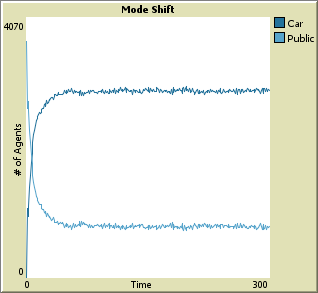
\includegraphics[width=8cm]{Simulation 1 mode shift}
\end{center}
\caption{Mode change proportions}
\end{figure}

\begin{figure}[h!]\label{f:32}
\begin{center}
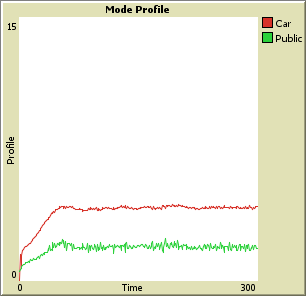
\includegraphics[width=8cm]{Simulation 1 mode profile}
\end{center}
\caption{Mode Profiles}
\end{figure}

\begin{figure}[h!]\label{f:33}
\begin{center}
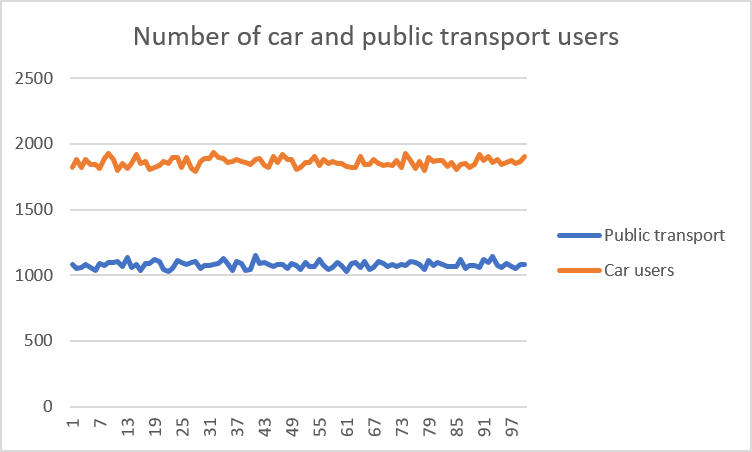
\includegraphics[width=12cm]{Simulation 2 Nocp}
\end{center}
\caption{Number of cars / public transport users}
\end{figure}

\begin{table}[h!]
\centering
\begin{tabular}{lllll}
\hline
\multicolumn{1}{l}{Travel mode} & \multicolumn{1}{l}{Average travel time} & \multicolumn{1}{l}{Average travel cost} & \multicolumn{1}{l}{Payoff} & Nash~ Equilibrium  \\ 
\hline
Car                             & 29.3                                    & 10                                      & 293                        & 0.23               \\
Taxi                            & 50                                      & 25                                      & 1250                       & 0.10               \\
Bus                             & 46                                      & 3                                       & 138                        & 0.31               \\
Rail                            & 59.8                                    & 4.5                           & 269.1                      
& 0.36                   
\end{tabular}
\caption{Nash Equilibrium of Travel mode choice game}
\label{table:2}
\end{table}

To find the Nash equilibrium, we can get it by averaging the travel time and cost then use the Nash equilibrium equations from 3.20 to 3.23 and calculate the payoff in equations from 3.1 to 3.4. The results are shown in table

When the structure of travel mode choice reaches Nash equilibrium values in Table \ref{table:2}, travel mode will remain stationary unless the payoffs of one or more mode parameters are changed. If a mode changes condition, a small perturbation appears. Then Nash equilibrium will be reached again after self adjusting.
\paragraph{}
Figure \ref{fig:31} represents the mode change proportions between car and public transportation over time observed after the first simulation of a 100 repetitions. While mode profiles are represented in Figure 3.5. The last figure 3.6 shows the changes in the number of car users versus the public transport users over time, after changing some of the characteristics of both modes such as public transport fares, car utility, and travel time.

It is important to note that in reality, traffic and weather conditions affect the payoff of travel by increasing the time of travel. Travelers tend to choose some modes because of its relatively stable travel time in weather conditions.
%\subsection{Model Validation}
%An important step in developing agent based models is to evaluate and validate the model carefully. Most models have several types of behaviors going at the same time, and it is important to understand what drives what and what affects what. Although our model is simple, it still needs to be validated and evaluated.


